\documentclass{article}
\usepackage[a4paper, total={180mm, 260mm}]{geometry}
\usepackage{graphicx}
\usepackage{url}
\usepackage{natbib}
\usepackage{todonotes}
\usepackage{booktabs}
\usepackage{lineno}
\usepackage{color}
%\usepackage{auto-pst-pdf}
\usepackage[colaction]{multicol}
\usepackage{caption}
\usepackage{svg}
\usepackage{authblk}
\usepackage{standalone}
\usepackage{xr}
\externaldocument{methods}

\usepackage[section]{placeins}


\linespread{1.5}

\makeatletter
\renewcommand{\maketitle}{\bgroup\setlength{\parindent}{0pt}
	\begin{flushleft}
		
		{\huge\textbf{\@title}}
		
		\bigskip
		
		{\large\textbf{\@author}}
		
		\bigskip
		
		{\large{Draft current \@date}}
		
	\end{flushleft}\egroup
}
\makeatother


% Title
\title{A Topic Model of Climate Change Literature}
\title{Words, words, words: Mapping the Matter of Climate Change Literature}
\title{A Topography of Climate Change Research}
\author[1,2]{Max Callaghan}
\author[1,2]{Jan Minx}
\author[2]{Piers M. Forster}

\affil[1]{Mercator Research Institute on Global Commons and Climate Change, Torgauer Straße, 10829 Berlin, Germany}
\affil[2]{Priestley International Centre for Climate, University of Leeds, Leeds LS2 9JT, United Kingdom}

\begin{document}
	\maketitle
	
	
	\begin{linenumbers}
		
		\noindent\textbf{\documentclass{article}

\begin{document}
	The massive expansion of scientific literature on climate change poses challenges for global environmental assessments and our understanding of how these assessments work. 
	Big data and machine learning can help us deal 
	with the large collections of text represented by scientific fields.
	Such methods help make the production of assessments
	more tractable, and give us better insights about how past assessments  have engaged with the literature as it has evolved.
	We use topic modelling to identify the thematic structure and draw a comprehensive topic map, or topography, of over 400,000 scientific publications from the Web of Science (WoS) on climate change. 
	We update current knowledge on the Intergovernmental Panel on Climate Change (IPCC), showing that, at least when compared to the baseline of the literature identified in the WoS,  the social sciences are in fact over-represented in recent assessment reports, and that
	technical, solutions-relevant knowledge - especially in the agricultural and engineering sciences - are under-represented.
	We point to a variety of other applications of such maps, and our findings have direct implications for addressing growing demands for more solution-oriented climate change assessments that are also more firmly rooted in the social sciences.
	We highlight fast-growing topics on solutions that could be better integrated into future IPCC reports. 
	The perceived lack of social science knowledge in solutions-relevant IPCC reports does not necessarily imply a bias towards the natural sciences. 
	It rather suggests a need for more social science research with a focus on ``technical'' topics related to climate solutions. 
\end{document}}
		
		
		
		\bigskip
		
		\noindent We live in an age of ``Big Literature'' 
		\cite{Nunez-Mir2016, Minx2017l}, where the science of climate change is expanding exponentially \cite{Grieneisen2011, Haunschild2016}. In the five years since the publication of the last IPCC assessment report \cite{IPCC2014c}, 202,000 papers on climate change were published in the Web of Science (WoS) (see Table \ref{tab}). This is almost as much as the 205,000 papers identified in the same query \cite{Grieneisen2011} during the first five assessment periods; a period of nearly 30 years. A total of around 350,000 new publications can be expected for before the sixth assessment report (AR6) of the Intergovernmental Panel on Climate Change (IPCC), based on current growth patterns (Figure \ref{pub-growth}). Moreover, the literature has also become more diverse. This is reflected in the expansion of the literature's vocabulary (see methods) - from 2,000 unique words in the first assessment period to 95,000 words so far in the sixth - indicating that the field has incorporated new content. For example, the zika virus, which was mentioned in 182 articles from 2014-2018, had never before been discussed in the titles or abstracts of articles relating to climate change. Yet it has emerged as a topic of high relevance: the incidence of the virus, the outbreak of which in Brazil in 2016 was declared a public health emergency by the World Health Organization, is set to increase under rising global temperatures \cite{Rao2019}. Similar rapid emergence patterns can be seen for Intended Nationally Determined Contributions (INDCs) and Sustainable Development Goals (SDGs) in AR6, and Biochar and the UN forest protection programme REDD in AR5, among others\footnote{The glossary in SI contains a complete list of the acronyms shown in the table}.
		
		\begin{figure}[htp]
			\begin{center}
				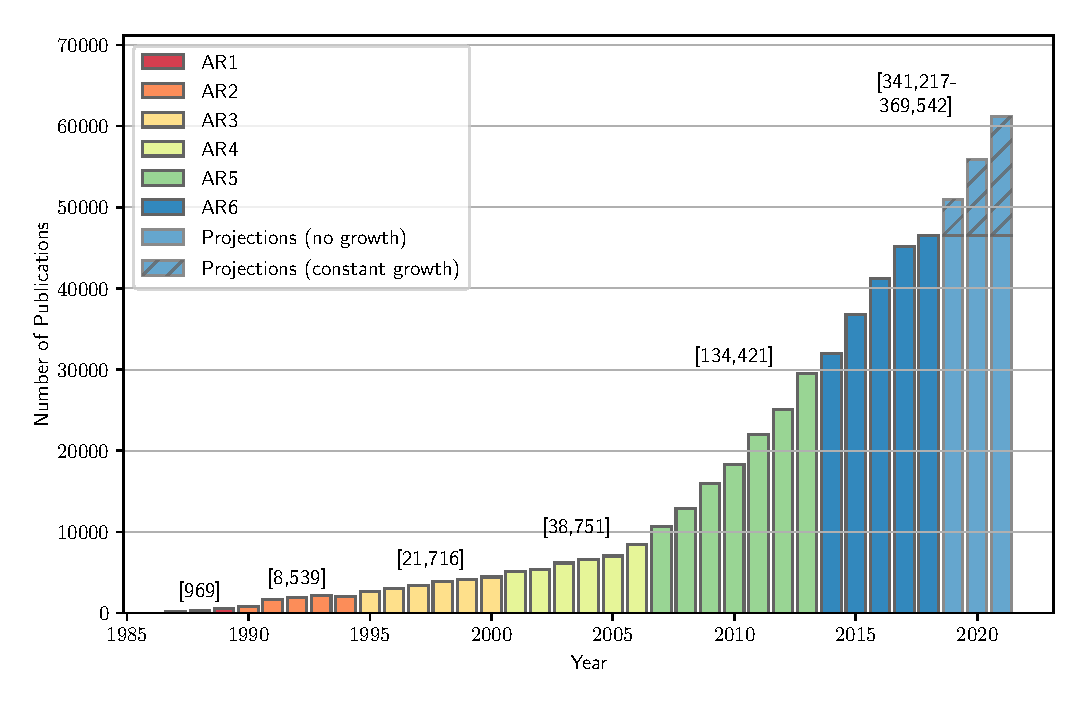
\includegraphics[width=180mm]{../plots_pub/pubs_time_wgb.pdf}
				\caption{ The number of climate change documents in the Web of Science in each year. A total of 406,191 documents were published until the end of 2018. The number of publications in each assessment period is shown in square brackets. For 2019-21 we project the number of papers assuming there is no more growth, and assuming that growth continues at the same rate as over the past five years}
				\label{pub-growth}
			\end{center}
		\end{figure}
		
		
		\begin{table}[htp]
			\begin{center}
				{\scriptsize
					\begin{tabular}{|l |p{1.8cm} p{1.8cm} p{1.8cm} p{1.8cm} p{1.8cm} p{1.8cm}|} 
\hline 
&\textbf{AR1} & \textbf{AR2} & \textbf{AR3} & \textbf{AR4} & \textbf{AR5} & \textbf{AR6}\\ \hline\textbf{Years} &1986-1989 & 1990-1994 & 1995-2000 & 2001-2006 & 2007-2013 & 2014-\\ 
\textbf{Documents} &1,167 & 8,539 & 21,716 & 38,750 & 134,413 & 201,606\\ 
\textbf{Unique words} &2,000 & 12,480 & 23,346 & 34,637 & 71,867 & 94,746\\ 
\textbf{New words} & change (560) & oil (287) & downscaling (217) & sres (234) & biochar (1,791) & mmms (313)\\ & climate (428) & deltac (283) & degreesc (187) & petm (95) & redd (1,113) & cop21 (234)\\ & co2 (318) & whole (256) & ncep (130) & amf (88) & cmip5 (679) & c3n4 (214)\\ & climatic (289) & tax (254) & fco (107) & sf5cf3 (86) & cmip3 (587) & sdg (187)\\ & model (288) & landscape (249) & pfc (98) & clc (81) & mofs (299) & zika (182)\\ & atmospheric (281) & alternative (243) & otcs (98) & embankment (81) & sdm (297) & ndcs (168)\\ & effect (280) & availability (242) & dtr (95) & cwd (79) & mof (275) & indc (164)\\ & global (224) & life (239) & nee (89) & etm (75) & biochars (252) & indcs (134) \\ \hline
\end{tabular}
}
				\caption{Growth of Literature on Climate Change. A glossary of acronyms is provided in SI}
				\label{tab}
			\end{center}
		\end{table}
		
		Big literature poses at least three challenges for scientific policy advice and science itself: \emph{First}, established procedures in scientific assessments like those conducted by the IPCC struggle to address the exploding literature base. For example, the ratio of studies cited in IPCC reports to the number of studies on climate change in the WoS has declined from 60\% to 20\%  \cite{Minx2017l}, posing a rapidly growing risk of selection bias. More generally, the exponential increase in the volume of literature means that the provision of comprehensive, objective, open and transparent assessments of the available scientific literature, as defined in the principles governing IPCC work \cite{IPCC2013}, is no longer possible for authors or author teams by traditional means. 
		Machine reading and learning methods as well as other data science applications are required to enable an understanding of the field of climate change research at scale. 
		\emph{Second}, evidence synthesis - the enterprise of reviewing the literature based on a formal and systematic set of methods \cite{Chalmers2002} - becomes increasingly important for aggregating and consolidating the rapidly emerging knowledge and enabling scientific assessments to do their job. 
		Yet traditional methods of evidence synthesis themselves are pushed to their limits by the large amount of scientific publications. The field of evidence synthesis technology, which tries to streamline human tasks through machine learning at the different stages of the review process, is still in its infancy \cite{Beller2018}. \emph{Finally}, overwhelming amounts of literature may be a major reason why studies of scientific assessments \cite{Bjurström2011, Hulme2010, Victor2015} do not offer robust quantification for their claims about the relationship between report citations and the underlying literature. 
		
		This study uses topic modelling \cite{Blei2010} to map out the vast body of evidence on climate change. Topic modelling is an unsupervised machine-learning technique, where patterns of word co-occurrences in documents are used to learn a set of topics which can be used to describe the corpus. The word topic derives from the Greek word for place (topos), and by \textit{situating} the documents in a reduced-form projection of their thematic content (see Figure \ref{oecd_topic_map}), we create a \textit{topographic map} of the literature on climate change. Such a systematic engagement with the thematic content of the climate science is missing from the literature so far. 
		We apply this map in a second step to understand how the IPCC reports have represented the available climate change literature and re-evaluate claims of bias based on a more comprehensive understanding of the available climate science. We enrich the discussion on representation in the literature by discussing topics as well as disciplines. 
		
		
		\subsection*{Mapping out the landscape of climate change literature}
		
		Figure \ref{oecd_topic_map} shows a \emph{thematic} or \emph{topographic map} of the 378,000 publications on climate change in our dataset that had abstracts with a total number of 140 topics. The number of topics must be defined exogenously, but the results are robust to different specifications. Using non-negative matrix factorization \cite{Lee1999}, the topics, which are groups of words that describe groups of documents, are machine-learned from the papers' abstracts (see methods for details, examples of different model specifications, and a thorough explanation of model selection). The topic scores of each document are reduced to the two dimensions shown through t-distributed stochastic neighbour embedding (t-SNE) \cite{vandermaaten2008}. \footnote{A full list of topics and related words, and a list of documents, their positions on the map, and their related topics are given in the SI}. The two dimensions represent a projection of the 140-dimensional topic scores of each document that seeks to preserve small distances between similar documents.
		
		
		\begin{figure}[htp]
			\begin{center}
				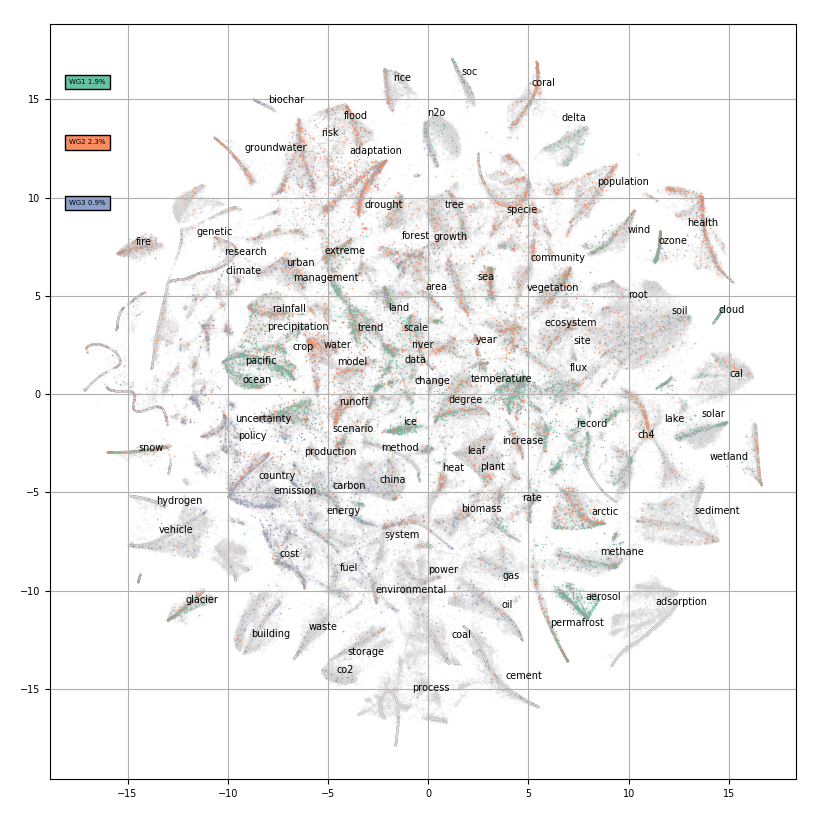
\includegraphics[width=180mm]{../plots_pub/all_topic_words_oecds.png}
				\caption{A map of the literature on climate change. Document positions are obtained by reducing the topic scores to two dimensions via t-SNE (see methods for further details). The two axes therefore have no direct interpretation, but represent a reduced version of similarities between documents across 140 topics. Documents are coloured by web of science discipline category. Topic labels are placed in the center of each of the large clusters of documents associated with each topic. }
				\label{oecd_topic_map}
			\end{center}
		\end{figure}
		
		
		
		The map shown covers a broad range of topics, with related topics shown in clusters. In general, topics related to climate science and impacts are on the left, while solution-oriented topics are on the right. More fine-grained research areas can also be distinguished. For example, publications related to urban infrastructure (\textbf{buildings}, \textbf{energy}, \textbf{cement}, \textbf{waste}) are located on the right, physical climate impacts such as \textbf{sea-level}, \textbf{droughts}  or [crop] \textbf{yield} are in the lower left and energy systems are in upper right. There are larger groups of documents at the fringes of the map that relate mainly to one or two specific topics such as \textbf{biochar}, \textbf{coral}, or \textbf{CO2 storage}. Interestingly, scenarios feature centrally in the map, at the interface between different scientific communities. This corresponds to their integrative nature in IPCC reports \cite{Moss2010}. This map of the thematic structure of the literature could be useful for individual scientific communities or for climate change assessments.
		
		
		The disciplinary composition of this research topography indicated by the different colours in Figure \ref{oecd_topic_map} highlights the dominance of natural sciences in climate change research. More than 60\% of the literature is published in natural science journals. Similarly, in 115 out of 140 topics the contribution of publications in natural science journals is greater than any other discipline. We calculate disciplinary entropy of topics as a measure of their degree of interdisciplinarity (see Figure \ref{dis-entropy} and methods for details). This shows how research on \textbf{health}, \textbf{food}, or \textbf{policy} comes from a range of disciplines, while research on \textbf{ice} and \textbf{oceans} comes almost exclusively from the natural sciences). 
		
		
		\begin{figure}
			\begin{center}
				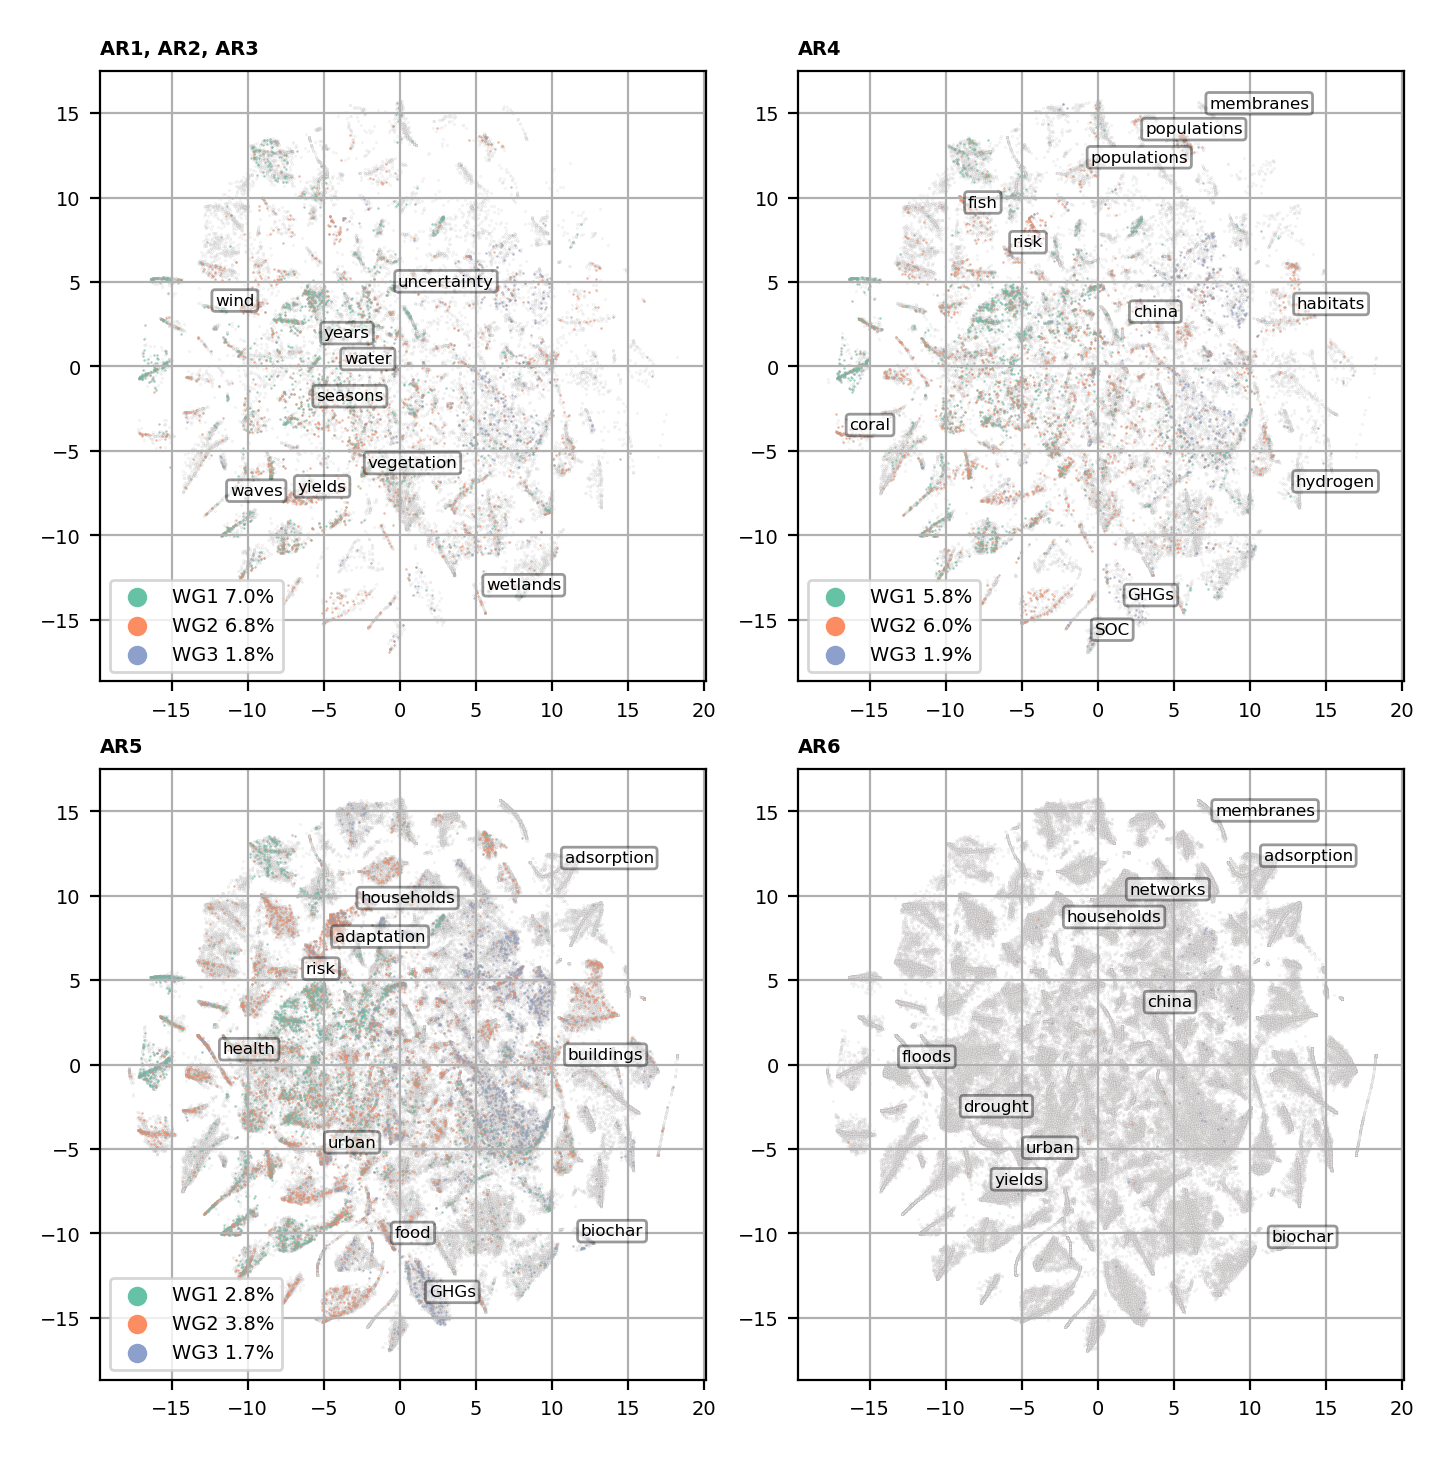
\includegraphics[width=180mm]{../plots_pub/topic_evolution_4.png}
				\caption{Evolution of the landscape of climate change literature. In each period, the 10 fastest growing topics are labelled. Where documents could be matched to IPCC citations, they are coloured by the working group citing them.}
				\label{evolution-map}
			\end{center}
		\end{figure}
		
		Finally, the topography shows the thematic evolution of the literature (Figure \ref{evolution-map}), with topics exhibiting distinct patterns of growth. Fast-growing topics in the last three assessment periods have included, among others, \textbf{coral}, \textbf{risks}, \textbf{adaptation}, \textbf{hydrogen}, \textbf{buildings}, \textbf{CO2 removal}, \textbf{networks} and \textbf{biochar}. \textbf{Biochar} is particularly remarkable in that the sizeable literature which emerged in AR5 was completely absent from the climate change literature beforehand. 
		The identification of new topics as they emerge, particularly as these are identified without prior knowledge of the literature, can help researchers and assessment-makers to keep abreast of a quickly evolving field.
		
		
		\subsection*{Research representation in IPCC reports}
		We apply our topic map to understand the representation of science in IPCC assesssments and how they manage to respond to demands for more solution-oriented knowledge \cite{Kowarsch2017}.  Several studies have identified, made, or repeated claims of a disciplinary bias of IPCC assessments towards the natural sciences, and within the social sciences towards economics \cite{Bjurström2011, Victor2015, Hulme2010, Corbera2016}. Where these claims were based on an analysis of IPCC citations \cite{Bjurström2011}, they fail to assess this claim against a measurable baseline. We argue here that this can be provided by the composition of the climate change literature as a whole. Although, as we discuss in the concluding section, it is in many ways imperfect, in view of the organisation's mandate to provide ``comprehensive, objective, open and transparent'' assessment of the available science \cite{IPCC2013}, our dataset of publications allows us to study representation with a meaningful baseline, and over time rather than for single assessment cycles. As such it forms a starting point for informed discussion about how to represent the literature according to the IPCC's priorities.  By matching the documents in our dataset to a set of references scraped from all published IPCC reports \cite{Minx2017l}, we can assess the representation of a group of studies by comparing the group's share in the subset of studies cited by the IPCC with it's share in the dataset of WoS studies on climate change (see methods for further details). 
		
		Figure \ref{oecd_rep}.a shows that the social sciences were indeed under-represented in the third assessment report, but by the fifth assessment report were over-represented. Likewise, social sciences other than economics have become better represented since AR3  (see figure \ref{subfield}f) with social \& economic geography (4.3\% of the literature), political science (1.0\%), and sociology (0.8\%) showing improved representation in AR5 compared to AR3, and social and economic geography, political science, and other social sciences better represented than economics. 
		
		This challenges what we think we know about the IPCC. The social sciences, by now, are actually the best represented field, with a share in the literature cited by IPCC reports 1.32 times higher than in the literature at large.  On the other hand the Agricultural Sciences and Engineering \& Technology have been consistently under-represented, with 2.27 and 3.49 times the share of studies in the wider literature than in the literature cited by the IPCC in AR5 respectively. Humanities are also under-represented, although they make up a very small proportion of the total literature.
		
		
		The topography allows us to delve deeper into the subject matter that receives more or less attention in the IPCC. Figures \ref{oecd_rep}b and \ref{oecd_rep}c plot the representation of the topics shown in the map. Figure \ref{oecd_rep}c shows that topics more commonly cited by IPCC working group I (WGI - the physical science basis) are older and largely better represented in IPCC reports. These topics, for example \textbf{ozone}, \textbf{oceans}, \textbf{clouds}, \textbf{aerosols} and \textbf{sea levels} make up some of the core topics of the physical science of climate change.
		
		The topics in the lower right of the graph are the most pertinent to the question of whether the IPCC is well representing knowledge on climate change. These topics are newer and until now have been under-represented in IPCC reports. Because they are new areas of knowledge, they may be highly salient in a periodic assessment process. These topics are primarily in working group III, on mitigation \footnote{see methods for a discussion of the categorisation of topics, including adsorption, and membranes, which may more properly be described as relevant to WGIII}.
		
		
		The difference between these under-represented new topics and other new topics that are better represented is intriguing. This difference is visible in figure \ref{evolution-map}, where in AR5, the clusters of documents around the \textbf{adsorption}, \textbf{buildings}, and \textbf{biochar} topics contain few IPCC citations, whereas the clusters around \textbf{food}, \textbf{health}, \textbf{adaptation}, and \textbf{GHGs} contain more. As shown in figure \ref{oecd_rep}c, \textbf{adsorption}, \textbf{buildings} and \textbf{biochar} are 4.08, 3.34 and 3.61 times more prevalent in the literature than in IPCC citations, while \textbf{food} is 1.22 times more prevalent in the literature and \textbf{health} and \textbf{adaptation} are 1.02 and 2.22 times more prevalent in IPCC citations respectively. The IPCC, has been better at integrating new knowledge from these topics, and in general better at integrating new knowledge from WG II than WG III topics.
		
		Further, within WG III topics, those that are well represented contain a greater proportion of social science research (figure \ref{oecd_rep}b). The topics \textbf{countries}, \textbf{policy}, and \textbf{prices} are close to a proportional representation and are made up of around 30\% social science research. \textbf{Waste}, \textbf{biochar}, \textbf{cement} and \textbf{coal}, are more than 3 times more prevalent in the wider literature than in the literature cited by the IPCC, and are made up of around 5\% social science research. This pattern is not visible in other working groups (see Figure \ref{socsci-wgs}), and complicates the perception of the under-representation of the social sciences.
		
		
		Recalling policymakers' demands for more solution-oriented assessments \cite{Kowarsch2017}, we could also interpret the topics that are newer and under-represented as ``solutions-relevant''. However, while policymakers' demands for solutions-oriented knowledge were rather about policy options, these under-represented new topics deal with more technical solutions and are found rather in technical disciplines within engineering \& technology and the agricultural sciences.
		
		\begin{figure}[htp]
			\begin{center}
				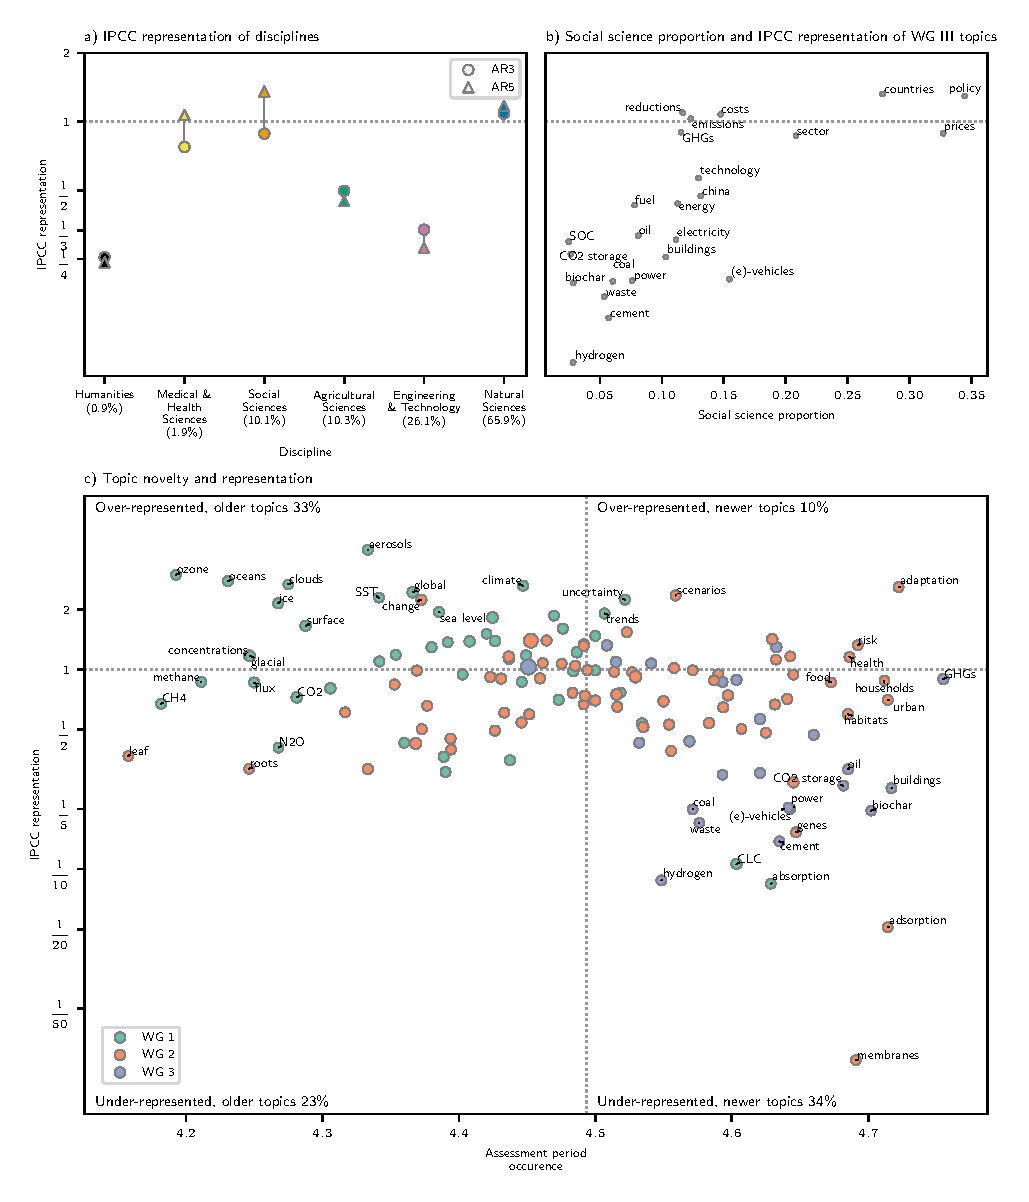
\includegraphics[width=180mm]{../plots_pub/big_panel_representation.pdf}
				\caption{Representation in IPCC reports: \textbf{a)} by discipline, \textbf{b)} by social science proportion of WG III topics, \textbf{c)} and novelty of all topics, where topics in the highest and lowest 10\% of either axis are labelled. Topics are coloured according to the working group from which they receive the most citations. Representation is the share of the subset of documents being cited by the IPCC divided by the share of the subset in the whole literature. We plot on a log scale so that 0.5 is equally distant to 1 as 2; plot labels show real values. Assessment period occurrence refers to the center of a topic's distribution across assessment periods (see methods for further details).}
				\label{oecd_rep}
			\end{center}
		\end{figure}
		
		
		\subsection*{Machine-learning for climate change assessments}
		
		
		We have shown that social science literature about climate change is over-represented in the IPCC, while technical literature on solutions is under-represented.
		A perfectly proportional representation of every part of the literature is of course not optimal, and a recommendation that the IPCC cite more of one part of the literature or less of another is by no means the goal of such an analysis. Indeed, the community of scientific experts made up by the IPCC is vastly better placed to decide on what is relevant, of high quality, and should be included in each report than any algorithm. 
		As with many machine learning applications, we should be mindful of David Hume's is-ought problem. 
		Machine learning can help us to more efficiently understand and describe the landscape of climate change literature, but we should be careful about what we interpret as a recommendation. In this light the two main results described here represent new knowledge about the interaction between the IPCC and the literature, which can have a variety of important implications. 
		The over-representation of the social sciences, combined with the perception that the IPCC needs to include more social science knowledge \cite{Victor2015}, suggests that doing so must involve the funding and production of more social science literature on climate change, not just greater efforts by the IPCC to include it. 
		Moreover, the fact that solutions-relevant topics are under-represented - while policymakers demand more solutions-oriented assessments - and that these topics contain little social science research, suggests areas where social science research may be usefully conducted, as well as opportunities for particularly fruitful interdisciplinary collaboration. Further, this fact can open a debate about the extent to which the IPCC should include more technical knowledge on solutions from disciplines within engineering and the agricultural sciences.
		
		
		The map can also serve as a guide to future assessments, to ensure that decisions about how different areas of the literature are represented are well-informed. 
		The map can contribute to these decisions as they are made from the scoping process, through to the selection by authors of individual studies.
		The advantage of topic modelling is that the outcome is not determined by any categorisation scheme imposed by the modeller, which facilitates the discovery of ``unsearched'' for topics. Highlighting recent research on, for example, membranes, biochar or e-vehicles, could prompt discussion in the scoping process about the extent to which each of these topics are relevant and should be included.
		This mode of discovery can act as a complement to human expertise, which may be better at identifying under-researched niches, existing biases or knowledge requirements.
		Beyond this, the methods shown here could aid other processes in the production of IPCC reports, such as the identification of potential authors to acheive a better balance across sectors, regions and genders \cite{Corbera2016}. The possible contribution of, or drawbacks to data science methods for IPCC processes is an important area for future research.
		Outside of the IPCC, this approach is part of ongoing attempts to make use of machine-learning within evidence synthesis. The topographic map presented is a new approach to rapidly mapping very large literatures. 
		
		The more than 400,000 publications we deal with here represent a wealth of knowledge on climate change and climate solutions. However, we acknowledge that our dataset is by no means exhaustive. We repeat an established query \cite{Haunschild2016}, granting that it may have imperfections. Beyond this we miss publications not in the Web of Science (some small journals, some books, and most grey literature, not to mention indigenous knowledge \cite{Ford2016b}); and studies relevant for the work of the IPCC, but that do not directly mention climate change (for example on energy policy). We argue that this remains a reasonable system boundary given data availability, and stress that the documents not included in our study alter our findings only if they have systematically different patterns of citation by the IPCC. In the future, making use of more sources of climate change knowledge, extracting and classifying information from full texts, or exploring author networks and interdisciplinarity, could improve the usefulness of this topography. Most importantly, machine learning applications should be explored that support IPCC authors in assessing the literature. This would prepare IPCC assessments for the age of big literature.
		
		
	\end{linenumbers}
	
	\appendix
	
	%\listoffigures
	\linespread{1}
	\bibliography{Mendeley}
	
	\bibliographystyle{unsrt}
	
	%	\documentclass{article}
\usepackage[a4paper, total={6in, 8in}]{geometry}
\usepackage{graphicx}
\usepackage{url}
\usepackage{natbib}
\usepackage{todonotes}
\usepackage{booktabs}
\usepackage{lineno}
\usepackage{color}
%\usepackage{auto-pst-pdf}
\usepackage[colaction]{multicol}
\usepackage{caption}
\usepackage{svg}
\usepackage{authblk}
\usepackage{standalone}
\usepackage[section]{placeins}

\makeatletter
\renewcommand{\maketitle}{\bgroup\setlength{\parindent}{0pt}
	\begin{flushleft}
		
		{\huge\textbf{\@title}}
		
		\bigskip
		
		{\large\textbf{\@author}}
		
		\bigskip
		
		{\large{Draft current \@date}}
		
	\end{flushleft}\egroup
}
\makeatother


\begin{document}
	% Title
	\title{A Topic Model of Climate Change Literature}
	\title{Words, words, words: Mapping the Matter of Climate Change Literature}
	\title{A Topography of Climate Change Research - Methods}
	\author[1,2]{Max Callaghan}
	
	\affil[1]{Mercator Research Institute on Global Commons and Climate Change, Torgauer Straße, 10829 Berlin, Germany}
	\affil[2]{School of Earth and Environment, University of Leeds, Leeds LS2 9JT, United Kingdom}
	\maketitle
	\begin{linenumbers}
	
	\setcounter{figure}{0}
	\renewcommand\thefigure{SI.\arabic{figure}}  
		
	\subsection*{Data}
	
	This study reproduces the query developed by \citep{Grieneisen2011}, which is carried out on the Web of Science core collection. Though not exhaustive, the Web of Science gives a good coverage of the literature in major peer-reviewed journals. The Web of Science data gives us a disciplinary classification (based on the journal) and publication year, among other metadata, for each document.	Each document is assigned to an assessment period according to the timeline shown in table 1.
	
	We use the references scraped from IPCC assessment reports from \citep{Minx2017l}, and attempt to match these with the results from the Web of Science. We use doc2vec similarity scores \cite{Le2014} to identify the 500 most similar titles for each reference, and count the document as a match if the jaccard similarity score of the two word shingles of the reference title and the document title is greater than 0.5 \cite{Khabsa2014}. Table \ref{ipcc-matching} shows the percentage of IPCC citations matched in each working group for each assessment report. This is significantly lower in earlier periods, as data coverage and quality of citation databases is lower for earlier periods. Matching in WG III is also lower, suggesting a greater share of non-peer review literature, or literature not directly mentioning climate change, but related to it's mitigation (for example on energy policy).
	
		\begin{table}[htp]
			\begin{center}
		\begin{tabular}{lrrrrr}
\toprule
AR &  1 &   2 &   3 &   4 &   5 \\
WG &    &     &     &     &     \\
\midrule
1  & 8\% & 25\% & 37\% & 47\% & 58\% \\
2  & 6\% & 12\% & 30\% & 38\% & 47\% \\
3  & 3\% &  9\% & 15\% & 22\% & 35\% \\
\bottomrule
\end{tabular}

	\caption{IPCC matching}
	\label{ipcc-matching}
	\end{center}
\end{table}
	
		
	\subsection*{Pre-processing}
	
	Data quality in earlier Web of Science results is poorer, and some documents have missing abstracts. In the quantification of the size of the literature and its vocabulary in table \ref{tab}, titles are substituted for abstracts where they are not available.  The words of the documents are lemmatized, replacing different forms of the same word (i.e. word/words) with a single instance. Commonly occurring words, or ``stopwords'' are removed, as are all words shorter than 3 characters, and all words containing only punctuation or numbers.
	
	The documents are transformed into a document-term matrix, where each row represents a document, and each column represents a unique word.  Each cell contains the number of that column's terms in that document. Only terms which occur more than once are considered.
	
	For the calculation of the topic model, documents with missing abstracts are ignored, and the document term matrix is transformed into a document
	frequency-inverse document frequency (tf-idf) matrix, where scores are scaled according to the frequency of their occurrence in the corpus. This gives more weight to terms which appear in few documents, and less weight to those which appear in many.
	
	\begin{equation}
	tf(t,d) = f_{t,d} \mathrm{,}\quad idf(t,D) = \log\frac{N}{|\{d \in D:t \in d\}|}
	\end{equation} 
	
	\subsection*{Topic Model}
	
	We use non-negative Matrix Factorisation (NMF) \cite{Lee1999}, an approach to topic modelling which factorises the term-frequency-inverse document frequency matrix \( V \) into the matrices \(W\), the topic-term matrix, and \( H \) the document-topic matrix, whose product approximates \(V\):
	
	\begin{equation}
		V_{i\mu} \approx (WH)_{i\mu} = \sum_{a=1}^{r}W_{ia}H_{a\mu}
	\end{equation}
	
	As demonstrated in Figure \ref{doc-topic}, each topic is represented as a set of word scores, and each document a set of topic scores. The combination of the two give the word scores in the document. For clarity in the figure, these are shown as simple counts, but in the model these are scaled according to each term's frequency within the corpus as explained above.
	
	Topics are calculated using the scikitlearn library \cite{Pedregosa2011}, and are saved in a database and topic visualisation system based on \cite{Chaney2012} \footnote{The system adds new functionality to \cite{Chaney2012} and combines it with a system for managing sets of documents and queries. The code and additional information is published online at \url{https://github.com/mcallaghan/tmv}}. 	
	
	\subsubsection*{Model selection}
	
	Topic models are calculated for 70, 80, 90, 100, 110, 120, 130, 140 and 150 topics. The run with 150 topics was discarded as it contained a topic to which no terms or documents were assigned. The relative usefulness of each model was assessed subjectively by the authors, based on inspection of the online visualisation tool, and the spreadsheet \textbf{topic\_comparison.xlsx} accompanying the supporting information. The spreadsheet shows each set of topics in adjacent columns. Topics from each model are placed next to the topics with the largest number of each topic's 10 highest scoring words in common. This helps authors to find an appropriate level of granularity for the analysis. 
			
	\subsubsection*{Topic Representation and Newness}
	
	To calculate topic representation in IPCC reports we divide each topic's share in the subsample of documents cited by IPCC reports by its share in the whole corpus. 
	
	We calculate a topic's total score as the sum of document-topic scores. A topic's window score is the sum of document-topic scores considering only documents in the given time window. To represent a topic's newness, we multiply each assessment period number by the share of it's total score occurring in that window, and take the mean of these scores. A topic in which 100\% of documents which make it up occurred in assessment period 1 (6) would thereby receive a score of 1 (6), while a topic evenly distributed across all assessment periods would receive a score of 3.5.
	
	
	\subsubsection*{Disciplinary Entropy}
	
	Disciplinary Entropy inverts the measurement of a conference's topical diversity suggested in \cite{Hall2008}, by measuring a topic \(z\)'s entropy \(H\), where 
	
	\begin{equation}
		H(f|z) = -\sum_{i=1}^K \hat{p}(f|z) \log \hat{p}(f|z) 
	\end{equation}
	
	based on the empirical distribution of a field \(f\) in the documents \(d\) in each topic:
	
	\begin{equation}
		\hat{p}(f|z) = \sum_{d:z_d=z} \hat{p} (f|d) \hat{p} (d|z)
	\end{equation}
	
	\subsubsection*{Topic Map}
	The topic model gives us the location of each document in a 140 dimensional topic space, with each dimension corresponding to a that document's \textit{topic-ness} in a given topic. t-Distributed Stochastic Neighbour Embedding (t-SNE) is a dimensionality reduction technique which we use to represent each document's topic scores in 2 dimensions \cite{vandermaaten2008}.

	\begin{figure}
		\begin{center}
			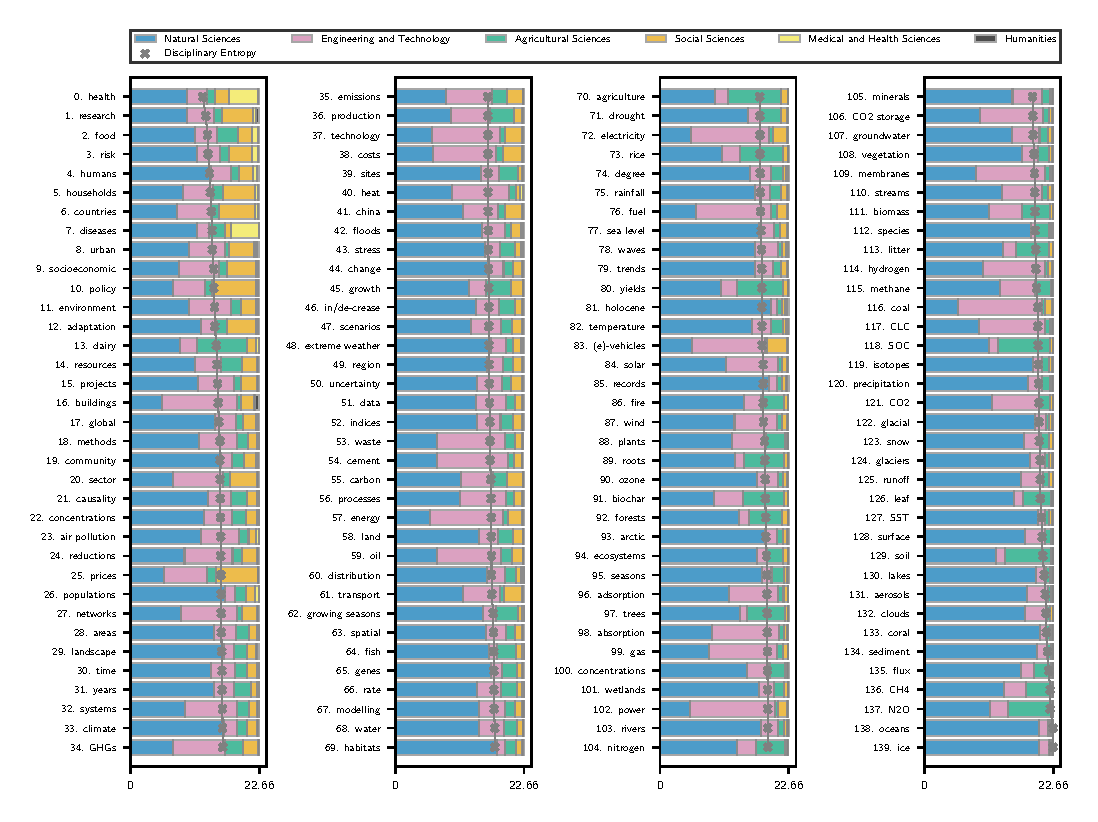
\includegraphics[width=1\linewidth]{plots_pub/topic_oecd_entropy.pdf}
			\caption{SI Disciplinary Entropy}
			\label{dis-entropy}
		\end{center}
	\end{figure}	
	
	
	
	\begin{figure}
		\begin{center}
			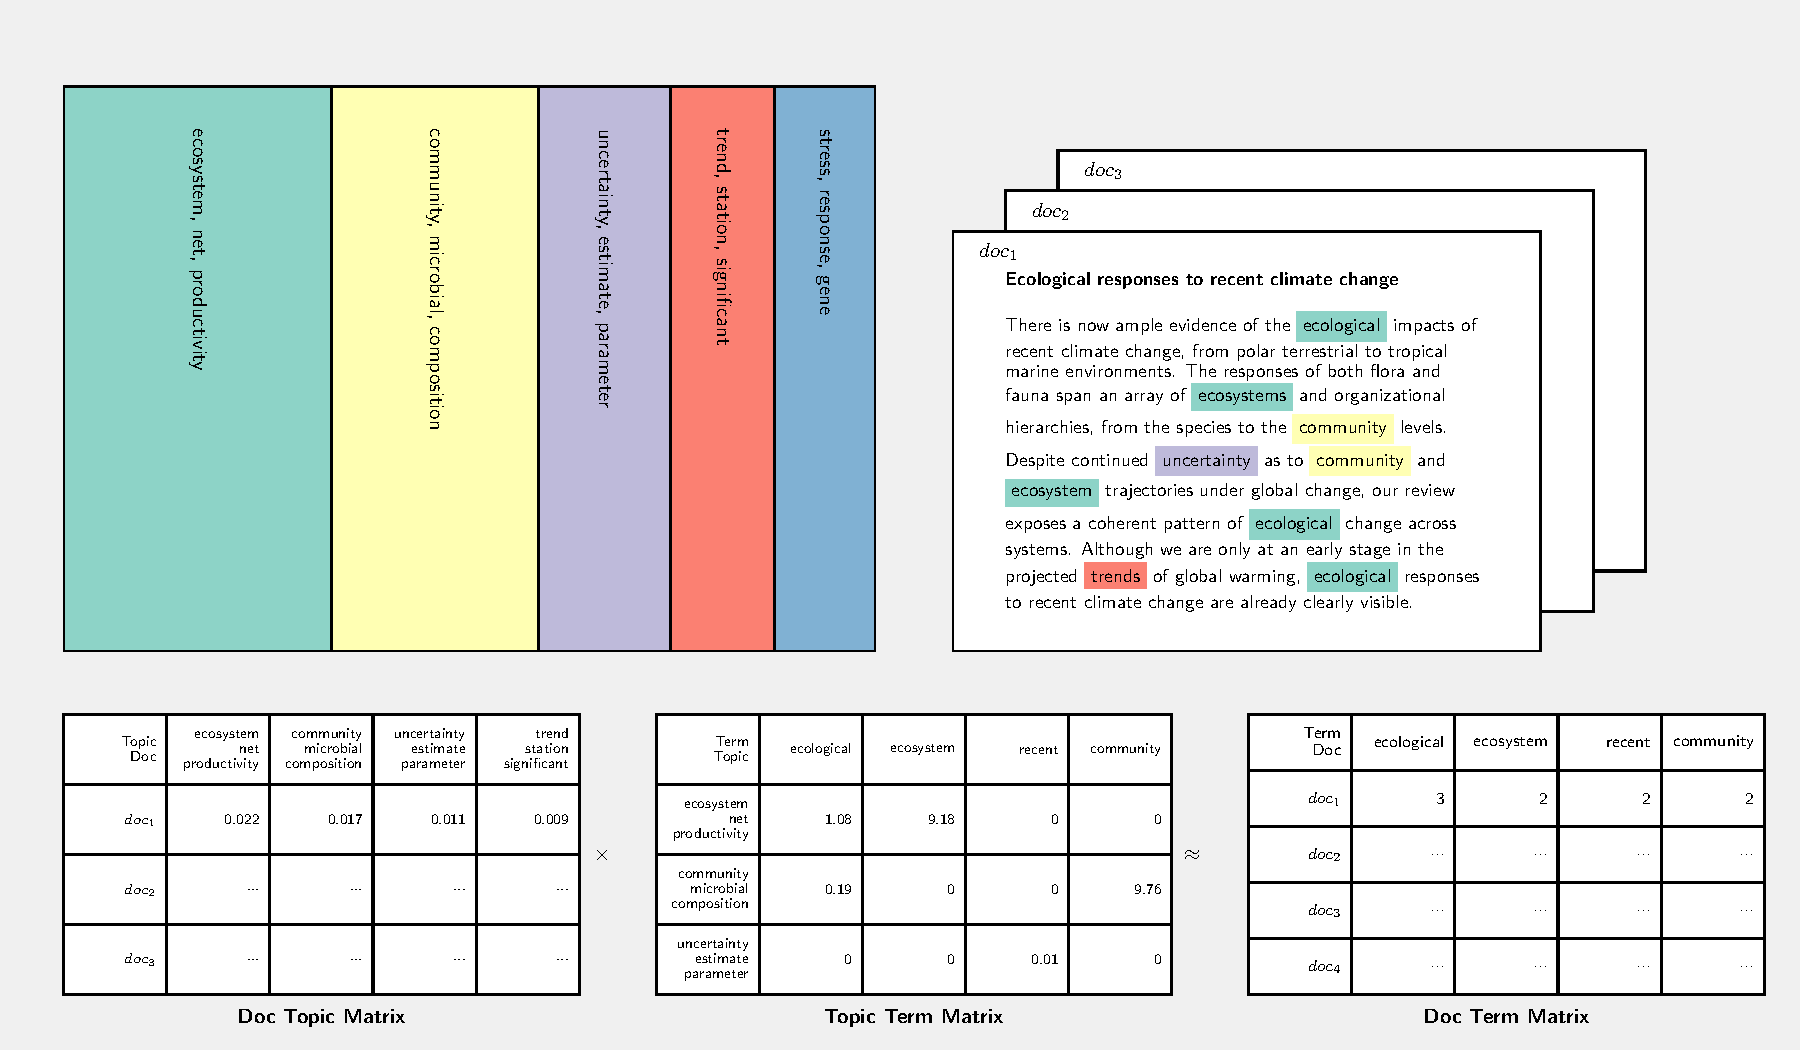
\includegraphics[width=1\linewidth]{plots_pub/single_doc_3_536594_1861.pdf}
			\caption{SI Topic make up of a single document}
			\label{doc-topic}
		\end{center}
	\end{figure}

	\begin{figure}
	\begin{center}
		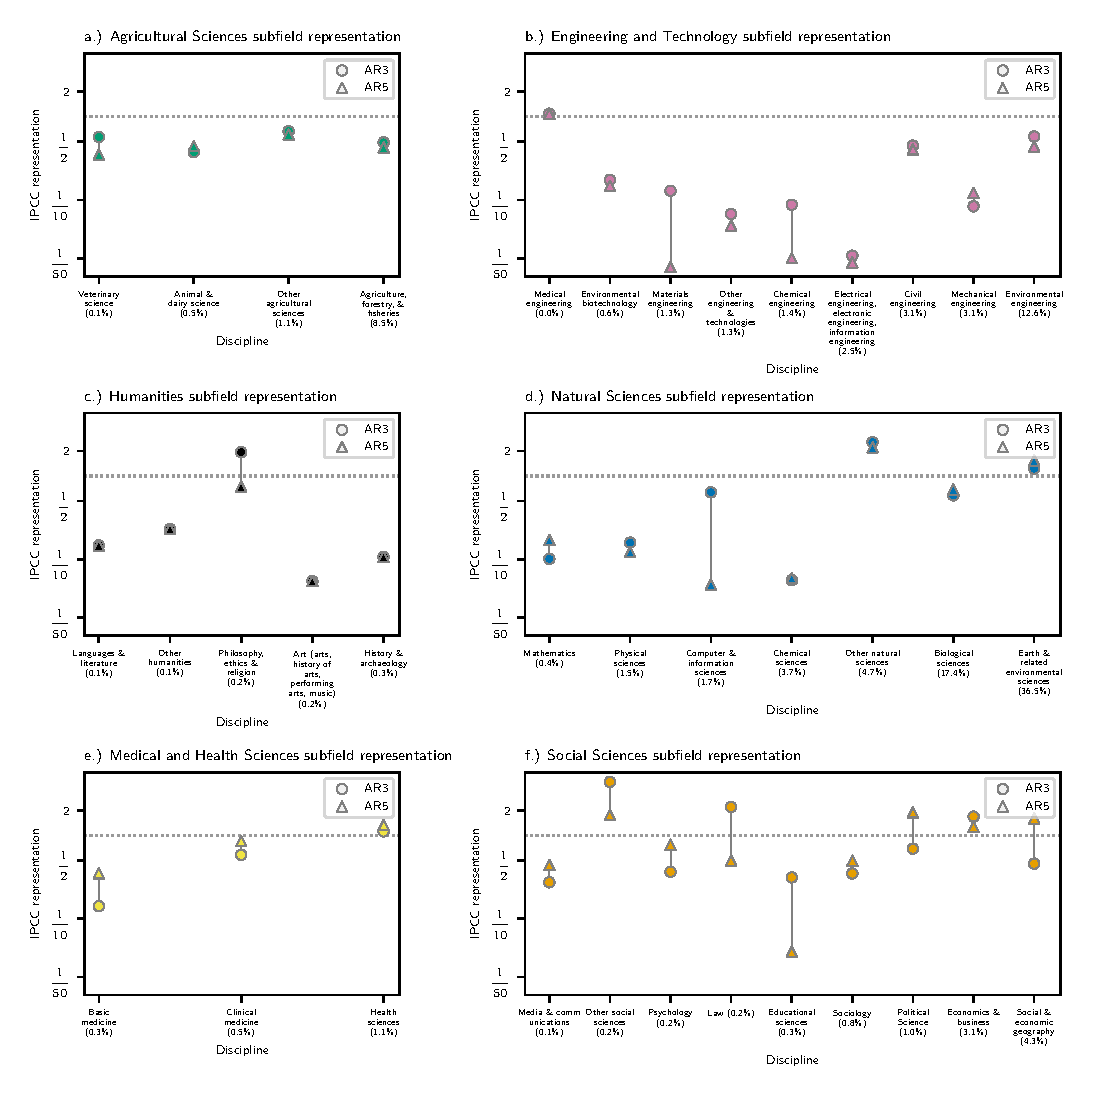
\includegraphics[width=1\linewidth]{plots_pub/ipcc_rep_wcs_simplified.pdf}
		\caption{SI Representation by subfield}
		\label{subfield}
	\end{center}
\end{figure}

\begin{figure}
	\begin{center}
		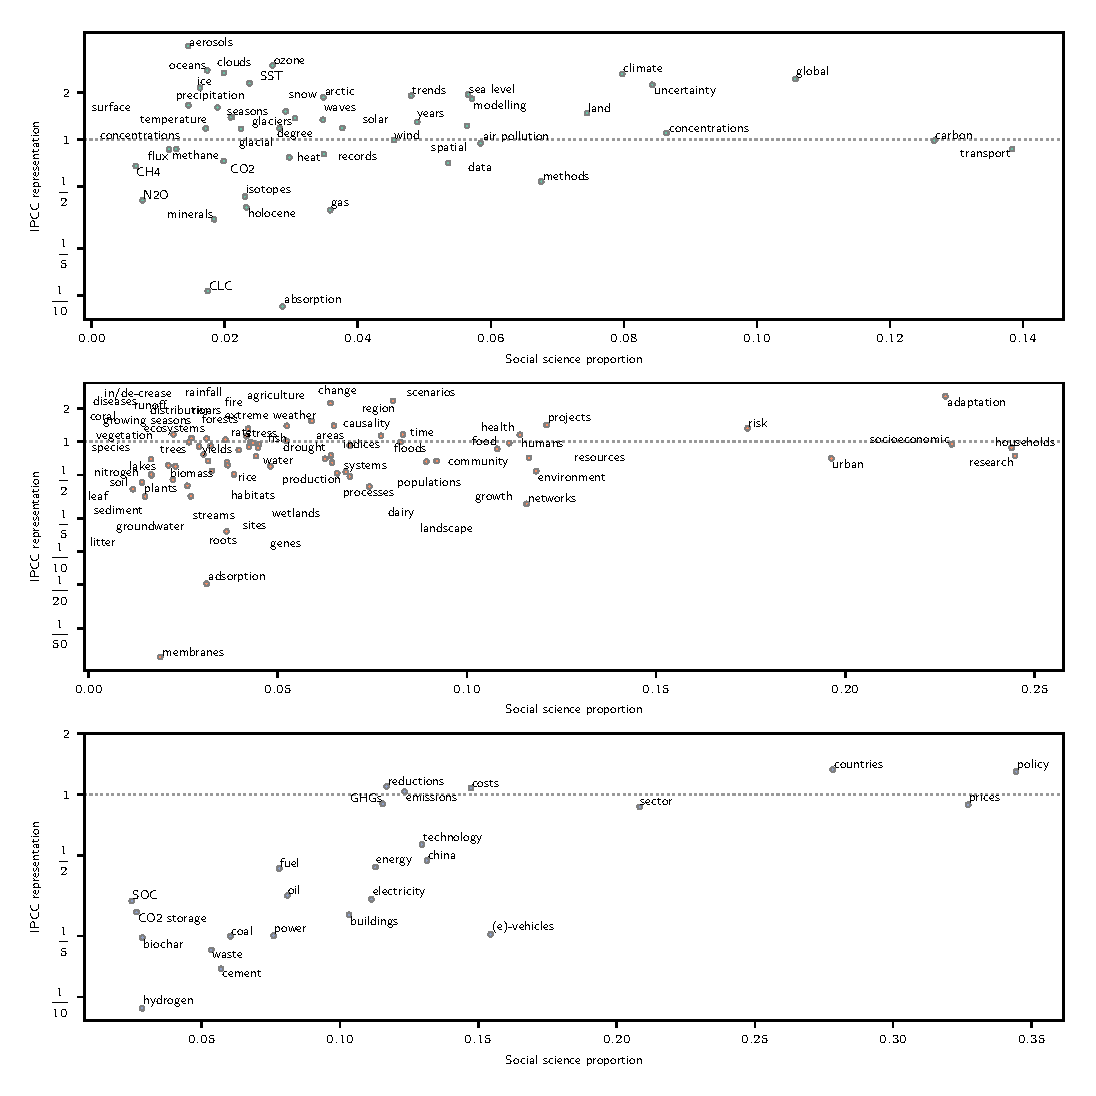
\includegraphics[width=1\linewidth]{plots_pub/wgs_socsci.pdf}
		\caption{SI Social science \& representation in topics across working groups}
		\label{socsci-wgs}
	\end{center}
\end{figure}

\begin{figure}
	\begin{center}
		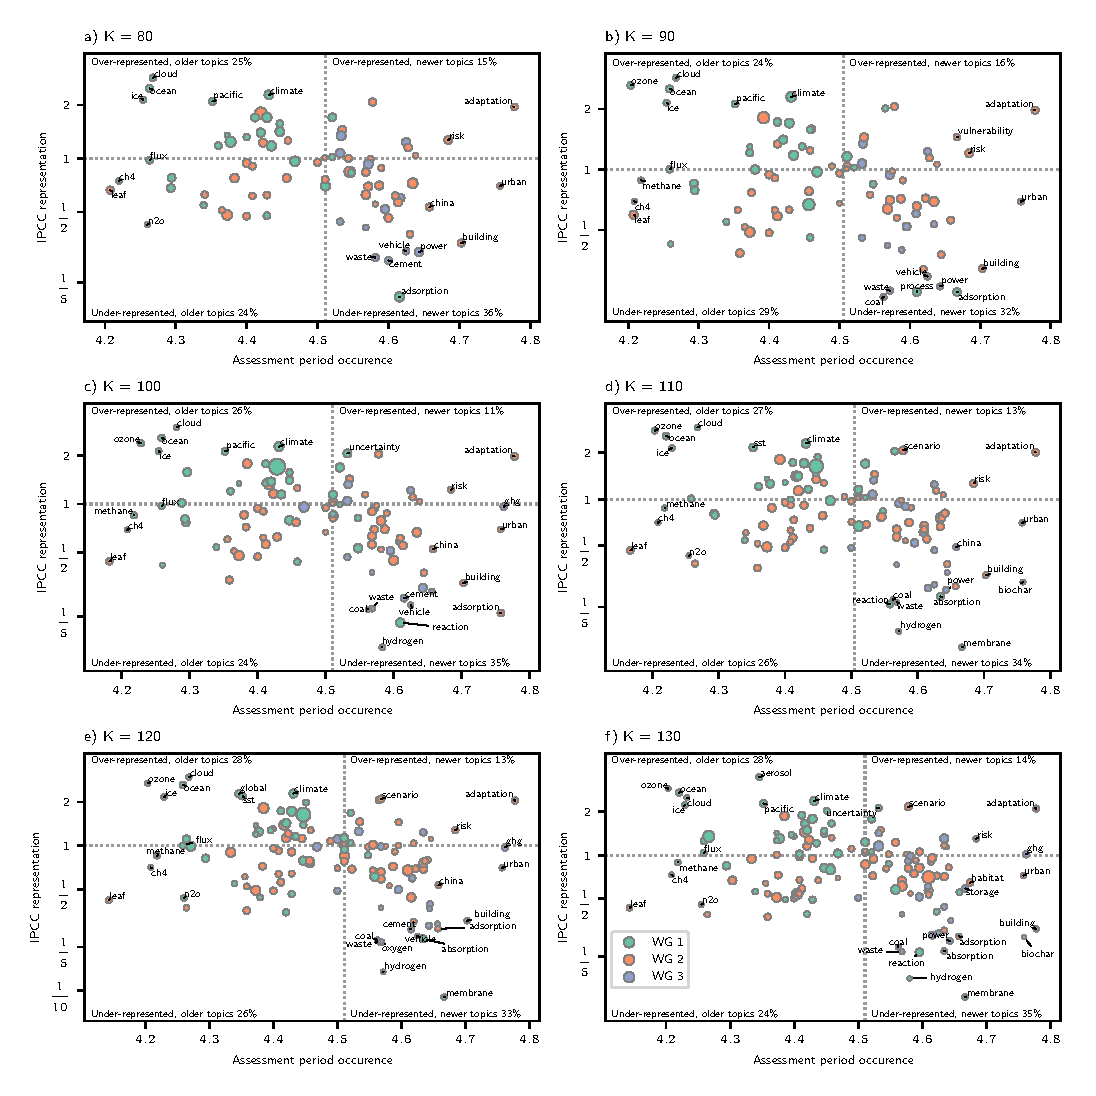
\includegraphics[width=1\linewidth]{plots_pub/topic_rep_ks.pdf}
		\caption{Topic representation over different values of K (number of topics). Topics in the upper or lower 6.66th percentile of either dimension are labelled}
		\label{top-rep-ks}
	\end{center}
\end{figure}

\subsection*{Glossary}


\noindent\textbf{ncep:} National Centers for Environmental Protection

\noindent\textbf{fco:} Fugacity of Carbon Dioxide

\noindent\textbf{pfc:} Perflourocompound

\noindent\textbf{otcs:} Open Top Chambers

\noindent\textbf{dtr:} Diurnal Temperature Range

\noindent\textbf{sres:} Special Report on Emissions Scenarios (200)

\noindent\textbf{petm:} Paleocene Eocene Thermal Maximum

\noindent\textbf{amf:}  Arbuscular Mycorrhizal Fungal

\noindent\textbf{sf5cf3:} trifluoromethyl sulfur pentafluoride (A Potent Greenhouse Gas Identified in the Atmosphere, 2000)

\noindent\textbf{clc:} Chemical Looping Combustion

\noindent\textbf{cwd:} Coarse woody debris

\noindent\textbf{etm:} Enhanced Thematic Mapper (NASA satellite sensor)

\noindent\textbf{cmip5:} Coupled Model Intercomparison Project 5 (Starting 2008)

\noindent\textbf{cmip3:} Coupled Model Intercomparison Project phase 3 (first published 2007 \cite{Meehl2007})

\noindent\textbf{mofs:} metal-organic frameworks (for CO2 storage)

\noindent\textbf{sdm:} statistical-dynamical model

\noindent\textbf{mmms:} Mixed Matrix Membranes (for CO2 capture)

\noindent\textbf{cop21:} 21st Conference of Parties (Paris 2015) 

\noindent\textbf{c3n4:} Carbon nitride (a synthetic nanomaterial used for hydrogen production)

\noindent\textbf{sdg:} Sustainable Development Goals

\noindent\textbf{indc:} Intended Nationally Determined Contributions

		
	\end{linenumbers}

\linespread{1}

%\bibliography{Mendeley}

\begin{thebibliography}{10}
	
	\bibitem{Grieneisen2011}
	Michael Grieneisen and Minghua Zhang.
	\newblock {The Current Status of Climate Change Research}.
	\newblock {\em Nature Climate Change}, 1:72--73, 2011.
	
	\bibitem{Minx2017l}
	Jan~C. Minx, Max Callaghan, William~F. Lamb, Jennifer Garard, and Ottmar
	Edenhofer.
	\newblock {Learning about climate change solutions in the IPCC and beyond}.
	\newblock {\em Environmental Science {\&} Policy}, 2017.
	
	\bibitem{Le2014}
	Quoc~V. Le and Tomas Mikolov.
	\newblock {Distributed Representations of Sentences and Documents}.
	\newblock {\em ICML}, 32, 2014.
	
	\bibitem{Khabsa2014}
	Madian Khabsa and C~Lee Giles.
	\newblock {The number of scholarly documents on the public web}.
	\newblock {\em PLoS ONE}, 9(5), 2014.
	
	\bibitem{Lee1999}
	D~D Lee and H~S Seung.
	\newblock {Learning the parts of objects by non-negative matrix factorization.}
	\newblock {\em Nature}, 401(6755):788--791, 1999.
	
	\bibitem{Pedregosa2011}
	Fabian Pedregosa, Ga{\"{e}}l Varoquaux, Alexandre Gramfort, Vincent Michel,
	Bertrand Thirion, Olivier Grisel, Mathieu Blondel, Peter Prettenhofer, Ron
	Weiss, Vincent Dubourg, Jake Vanderplas, Alexandre Passos, David Cournapeau,
	Matthieu Brucher, Mattheiu Perrot, and {\'{E}}douard Duchesnay.
	\newblock {Scikit-learn: Machine Learning in Python Fabian}.
	\newblock {\em Journal of Machine Learning Research}, 12:2825--2830, 2011.
	
	\bibitem{Chaney2012}
	Allison J~B Chaney and David~M. Blei.
	\newblock {Visualizing Topic Models}.
	\newblock {\em Icwsm}, pages 419--422, 2012.
	
	\bibitem{Hall2008}
	David Hall, Daniel Jurafsky, and Christopher~D. Manning.
	\newblock {Studying the history of ideas using topic models}.
	\newblock {\em Proceedings of the Conference on Empirical Methods in Natural
		Language Processing - EMNLP '08}, pages 363--371, 2008.
	
	\bibitem{vandermaaten2008}
	Laurens van~der Maaten and Geoffrey Hinton.
	\newblock {Visualizing Data using t-SNE}.
	\newblock {\em Journal of Machine Learning Research}, 9:2579--2605, 2008.
	
	\bibitem{Meehl2007}
	Gerald~A. Meehl, Curt Covey, Thomas Delworth, Mojib Latif, Bryant McAvaney,
	John~F.B. Mitchell, Ronald~J. Stouffer, and Karl~E. Taylor.
	\newblock {The WCRP CMIP3 multimodel dataset: A new era in climatic change
		research}.
	\newblock {\em Bulletin of the American Meteorological Society},
	88(9):1383--1394, 2007.
	
\end{thebibliography}

\bibliographystyle{unsrt}

\end{document}
	
\end{document}